\chapter{全景漫游的交互模型}
全景漫游中的用户交互属于典型的多通道交互,根据前文所列举的关于人的意识的相关理论可知,人在面对多通道输入的刺激时,会或主动或被动地选择一种进行注意。如果这些刺激可以达到被人记忆并在需要时主动唤起的效果,那有可能在多通道输入中自动加工处理,减少对人的脑力资源的占用。同时,经过良好规划的交互模型也能避免用户出错的概率,提高网络资源的利用率,降低后台服务器程序处理的负担。

基于上述假设,尝试通过认知理论对全景漫游中设备端交互、菜单交互和场景交互,分别构建交互模型。以期通过多种形式展现信息,达到更高效表达场景的意图,结合人与设备的关系切实提升用户操作体验。

\section{设备交互}
交互从人发出的信息至被设备捕获转换为数字信号是一个明显的“编码/解码”的过程。人的动作相当于人通过分析相关信息,并试图理解机器的运作模式,认识到自己所需表达的信息,最后发出了一个按照“所认为机器能够理解的方式”进行编码的“信号”。而设备则是处在各种信息的海洋中,一刻不歇地从外界收集信息,当成功捕获到一个匹配其预设规律的“信号”时,通过确定的解码方式,还原出人最初想表达的信息。

\subsection{信息流与反馈等待}
设备无时无刻不在等待着用户的信息输入,而用户的输入是多通道的,在不同的通道上都会捕获到用户的输入流。多输入流经过处理后在主信息流上合并成一条输入流,由设备程序进行集中处理。如图\ref{fig:reactive}。

\begin{figure}[htp]
\centering
\fbox{
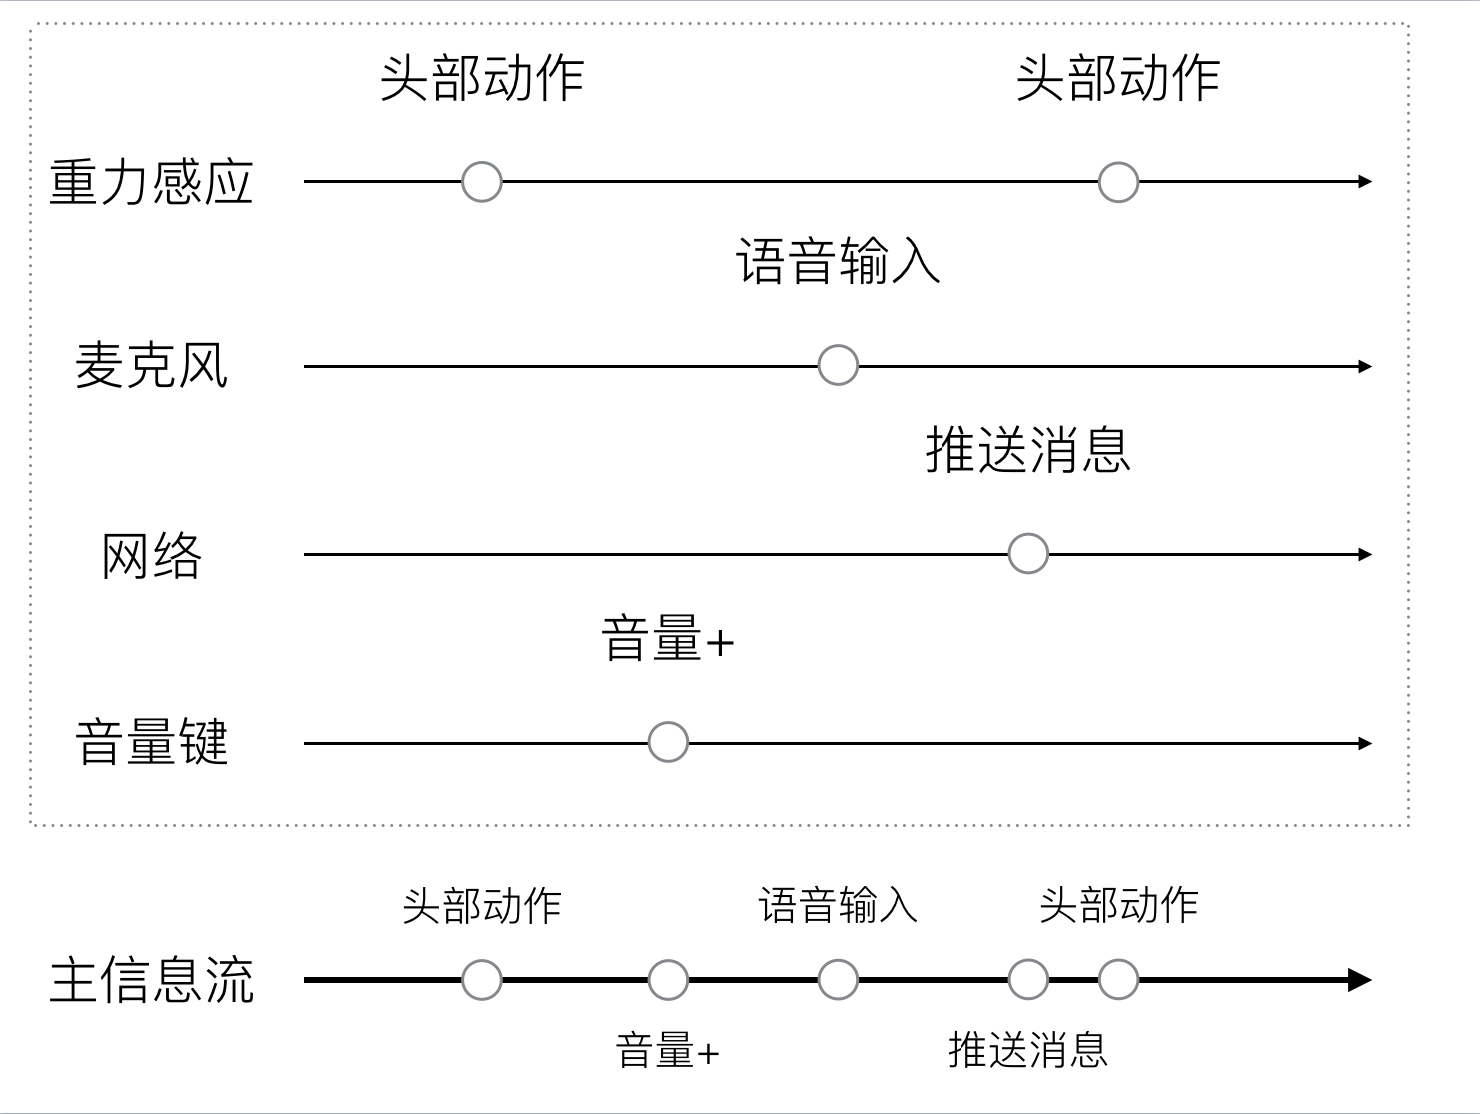
\includegraphics[width=.5\textwidth]{reactive}
}
\caption{信息流}
\label{fig:reactive}
\end{figure}

但常见的场景是,交互行为的发生与处理完成得到反馈并不是即时的,而要经过一定的时间,其等待时间因网络延迟或设备响应而不一。这时用户等待的过程就会形成一阵交互效果上的“盲区”,也就是常见的“设备无响应”状态,如图\ref{fig:stream}	。“设备无响应”情形在一般设备上出现并不会造成过大的后果,但是在全景漫游中用户的视野处在封闭的空间中,长时间得不到合理反馈易造成用户心理恐慌,是需要通过设计极力避免的情形。

\begin{figure}[htp]
\centering
\fbox{
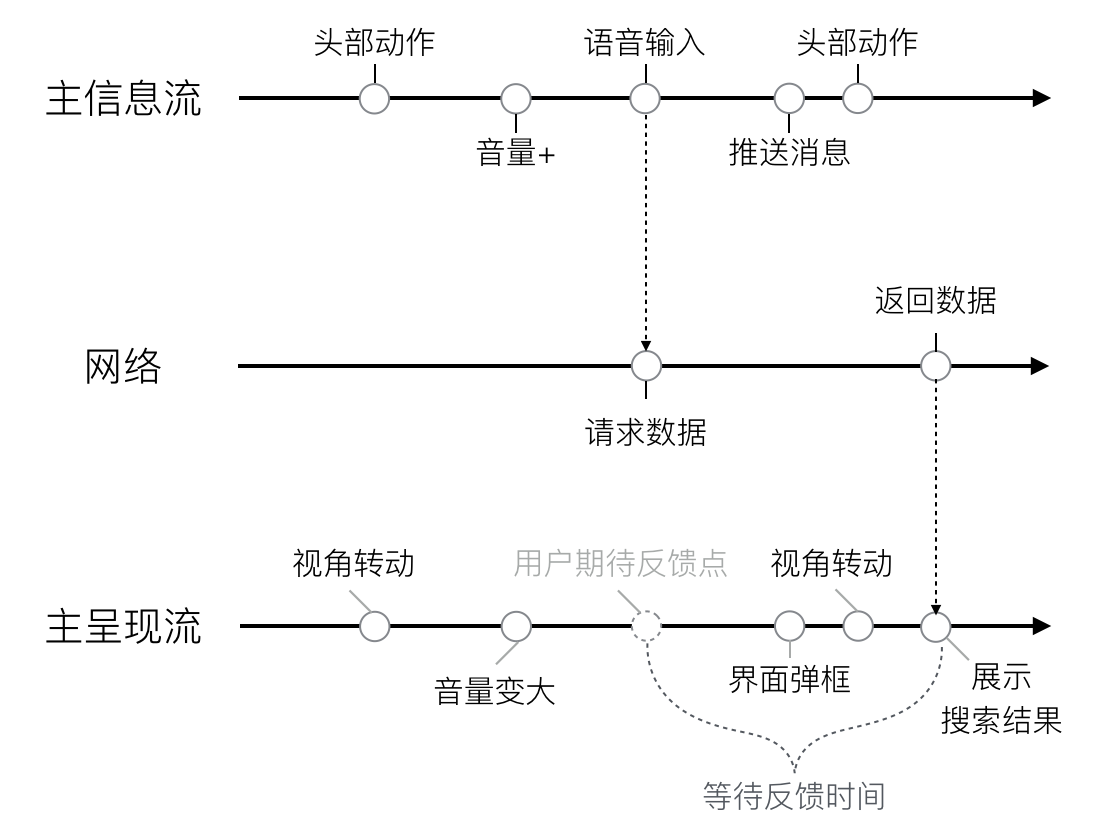
\includegraphics[width=.5\textwidth]{stream}
}
\caption{交互中因其他元素造成的等待}
\label{fig:stream}
\end{figure}

即时反馈信息是最理想的方案,但现实情况必须对此作出解释以避免用户等待无反馈而产生迷茫情绪。常见的方案是对用户的输入做出即时反馈,当反馈不能即时给到时给出等待反馈的提示。前文所提到的通过注视(gaze)一定时间而做出确定选择的过程就是一种非即时的操作,在等待确认完成过程中通过一些标示告知用户:此处正在等待完成的行为是什么,预计完成的时间是多少等。

\subsection{信息修正}
信息流的出现帮助解决了信息加工过程中信息传达时间不一致的问题,但用户有可能得到的信息不准确或是很模糊,需要用户去判断信息是否符合预期,在无法判断信息的有效性时,如果能够提供给用户一个可以自我纠正的语境,将有利于用户自己辨别信息\endnote{路璐,田丰,戴国忠,王宏安. 融合触、听、视觉的多通道认知和交互模型[J]. 计算机辅助设计与图形学学报,2014,(04):654-661.}。

例如,在导航过程中提供给给用户当前朝向与正确方向的箭头图示,用户会尝试向左或向右转向,当向左转时会发现偏离变大,而向右转时会发现偏离变小,用户自然会选择向右转以回到正确方向上去,如图\ref{fig:correct}。

\begin{figure}[htp]
\centering
\fbox{
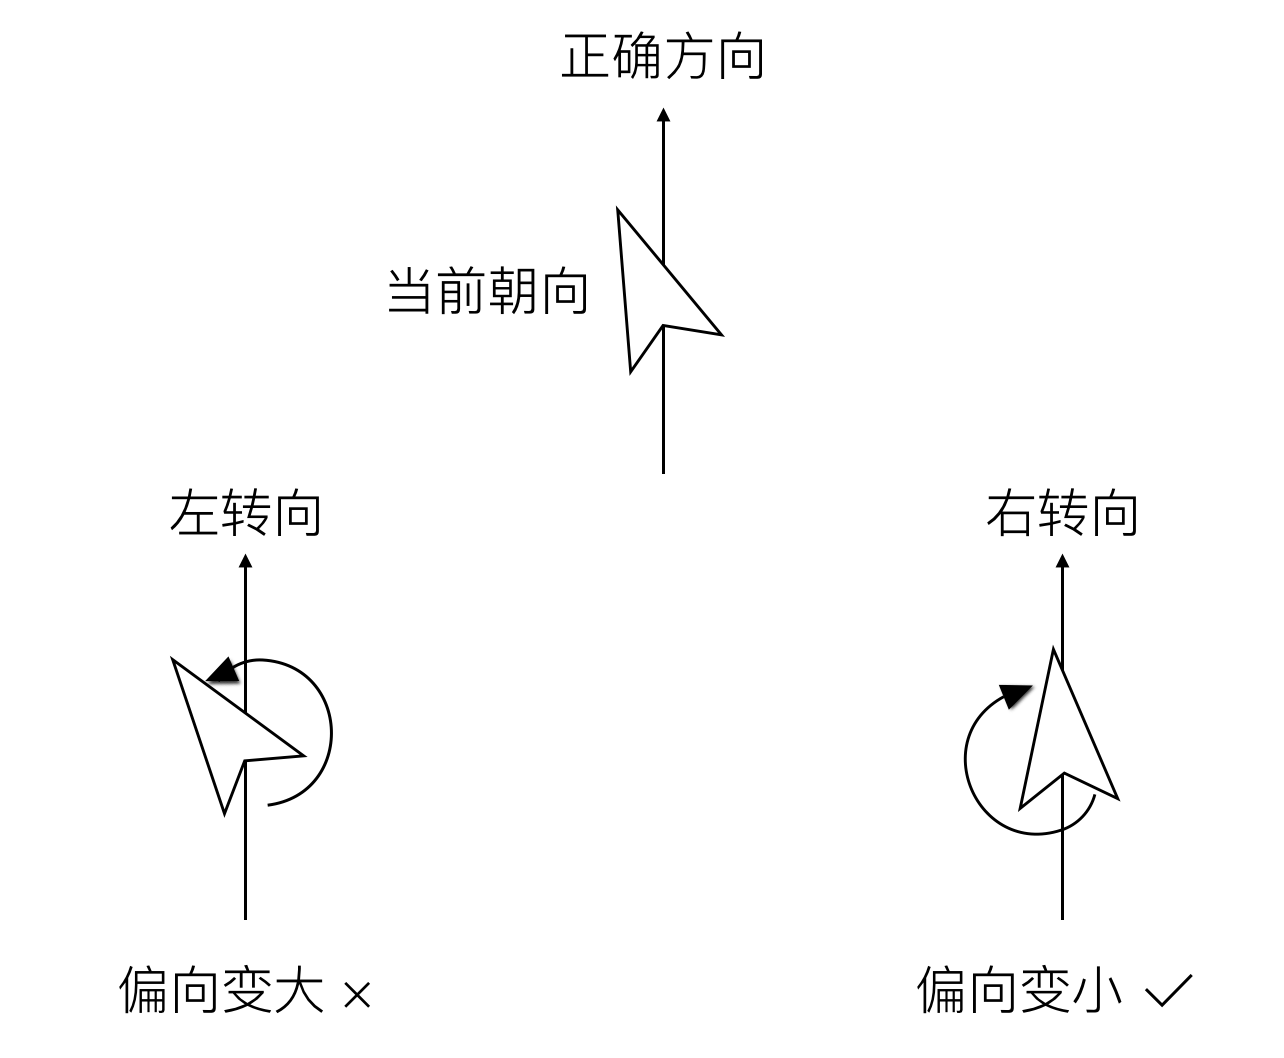
\includegraphics[width=.5\textwidth]{correct}
}
\caption{自我修正的交互行为}
\label{fig:correct}
\end{figure}

在全景漫游中与设备进行多通道交互是可行且必要的,人的感官可以从不同通道间获取信息,使人获得的信息更为全面。更为关键的是多通道信息往往能够起到互补的作用,使得信息交互的鲁棒性大大提高,也使用户对于系统和环境的适应性得到了提升。而全景漫游因与普通的设备交互有所不同,故应加强信息流的建立,避免用户无谓的等待,提高交互的流畅性。而在交互的结果上注重信息的可修正性,帮助用户通过自我反馈建立准确有效的信息流。

\section{导航交互}
全景漫游中导航功能的重要性不言而喻,但场景中元素的可识别要求又限制了导航功能的复杂度。导航应符合用户对信息整合的需求,而又对场景内容起烘托作用。由前一章信息架构的组织形式可知,导航应包括自顶向下、自底向上、不可见联结这三种基本信息组织形式,它们分别体现为导航层级的上下文感知、单个内容增强信息展示和多任务切换。

\subsection{上下文感知}
上下文是指当前环境中区别于当前本体的因素。上下文按与用户关系可简单分为主动上下文和被动上下文两种。主动上下文指环境中可以直接改变系统行为的状态或变量。被动上下文指那些虽不能直接产生作用但可引起用户兴趣继而通过用户改变系统行为的状态或变量\endnote{张磊. 上下文感知在导游系统中的应用[A]. 中国计算机学会、中国图象图形学学会、ACM SIGCHI中国分会、清华大学计算机科学与技术系.第一届建立和谐人机环境联合学术会议(HHME2005)论文集[C].中国计算机学会、中国图象图形学学会、ACM SIGCHI中国分会、清华大学计算机科学与技术系:,2005:4.}。上下文感知是指计算实体能够根据上下文环境的变化及时调整自身行为,使用户从信息的管理和输入中解放出来,专注于要执行任务的本身\endnote{王守芳, 金浩, 魏鲲,等. 上下文感知综述[C]// 建立和谐人机环境联合学术会议. 2005.}。

上下文感知的作用非常重要,没有上下文用户很难预计进行操作时即将发生的变化,容易在使用过程产生困惑。在通过列表批量展示内容时都会同时展示该内容的多项信息,包括名称、录入时间、信息量等(可能因内容类型不同而信息名称有所差异)。例如商城类网页会展示商品的名称、产地、出厂时间等,这些信息就是上下文。通过阅读理解相关信息,用户可以在不打开具体页面的情况下对相应项目得到一个基本的认识。

\subsection{增强信息}
在单个页面里尽可能多地铺陈相关信息,包括其他相关内容,减少用户反复查找的负担。

\subsection{多任务切换}
类似 MacOS 的最大化最小化。

\section{场景交互}

\subsection{直观的交互}
WYSIWYG,即“所见即所得”是一种常见的编辑模式,它便是一种很理想的设备交互模型,用户不必关注程序背后的逻辑,甚至不必关心自己编辑的文章真实存储的数据是何种形式,只需要看到屏幕上呈现的内容就是别人所能看到的内容。

全景漫游展示的正是这样一种过程,由不直观的概念转换为直观的概念。如图\ref{fig:wysiwyg}所示,人对房屋整体概念的认识观念是从具象至抽象,只有抽象简洁的概念才能方便地存储于人脑的记忆中,但涉及到具体房屋的理解时,是从单纯的“房屋”名词,到草图的展示,再到带有色彩的照片。而全景漫游要实现的是一个身临其境的房屋场景,是比照片更贴近真实房屋的信息载体。全景漫游的内容注重交互形式和体验感受的留存,不注重内容的记忆,故直观的交互符合其交互需要。

\begin{figure}[htp]
\centering
\fbox{
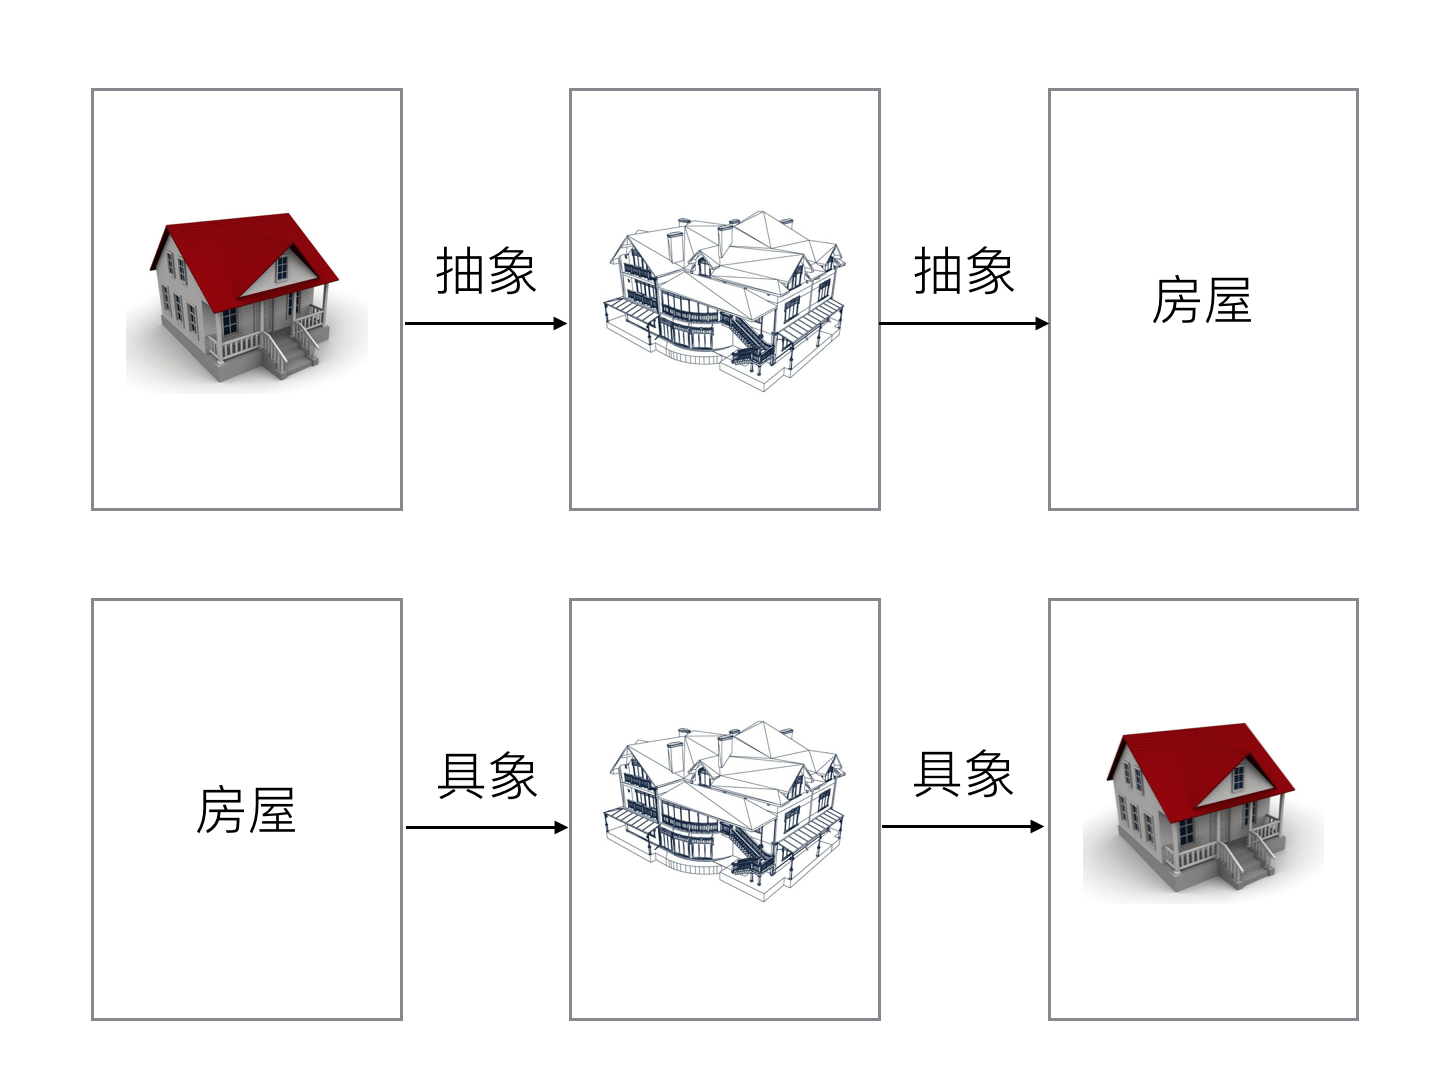
\includegraphics[width=.5\textwidth]{wysiwyg}
}
\caption{具象和抽象}
\label{fig:wysiwyg}
\end{figure}

\subsection{熟悉的定位点}
游戏中我来过的地方可以作为参照物。